\documentclass[a4paper, 12pt]{article}
\usepackage{titling}
\usepackage{array}
\usepackage{booktabs}
\usepackage{enumitem}
\usepackage{graphicx}
\usepackage{hyperref}
\usepackage{amssymb}
%\usepackage{mathtools}
\usepackage{listings}
\usepackage{amsmath}
\usepackage{color} %red, green, blue, yellow, cyan, magenta, black, white
\setlength{\heavyrulewidth}{1.5pt}
\setlength{\abovetopsep}{4pt}
\setlength{\parindent}{0pt}
\graphicspath{{.}}
\usepackage{float}
\usepackage[margin=1in]{geometry}
\definecolor{mygreen}{RGB}{28,172,0} % color values Red, Green, Blue
\definecolor{mylilas}{RGB}{170,55,241}
% Must be after geometry
\usepackage{fancyhdr}
\pagestyle{fancy}
\fancyhf{}
\rhead{NN Homework 7}
\lhead{P.Lukin, E. Ovchinnikova}
\cfoot{\thepage}

\setlength{\droptitle}{-5em}

\title{Neural Networks  \\
				- Homework 7 -}
\author{Petr Lukin, Evgeniya Ovchinnikova}
\date{Lecture date: 14 November 2016}

\begin{document}

%-------------------------------------------------------------------------------
\lstset{language=Matlab,%
    %basicstyle=\color{red},
    breaklines=true,%
    morekeywords={matlab2tikz},
    keywordstyle=\color{blue},%
    morekeywords=[2]{1}, keywordstyle=[2]{\color{black}},
    identifierstyle=\color{black},%
    stringstyle=\color{mylilas},
    commentstyle=\color{mygreen},%
    showstringspaces=false,%without this there will be a symbol in the places where there is a space
    numbers=left,%
    numberstyle={\tiny \color{black}},% size of the numbers
    numbersep=9pt, % this defines how far the numbers are from the text
    emph=[1]{break},emphstyle=[1]\color{red}, %some words to emphasise
    emph=[2]{end,function}, emphstyle=[1]\color{blue},
}

%-------------------------------------------------------------------------------

\maketitle

\section{Mind map}

\begin{figure}[h]
  \centering
  \caption{Mind map. Chapter 5 from Haykin's book. A zoomed version is attached as Radial-BasisFunctionNetworks.png}
  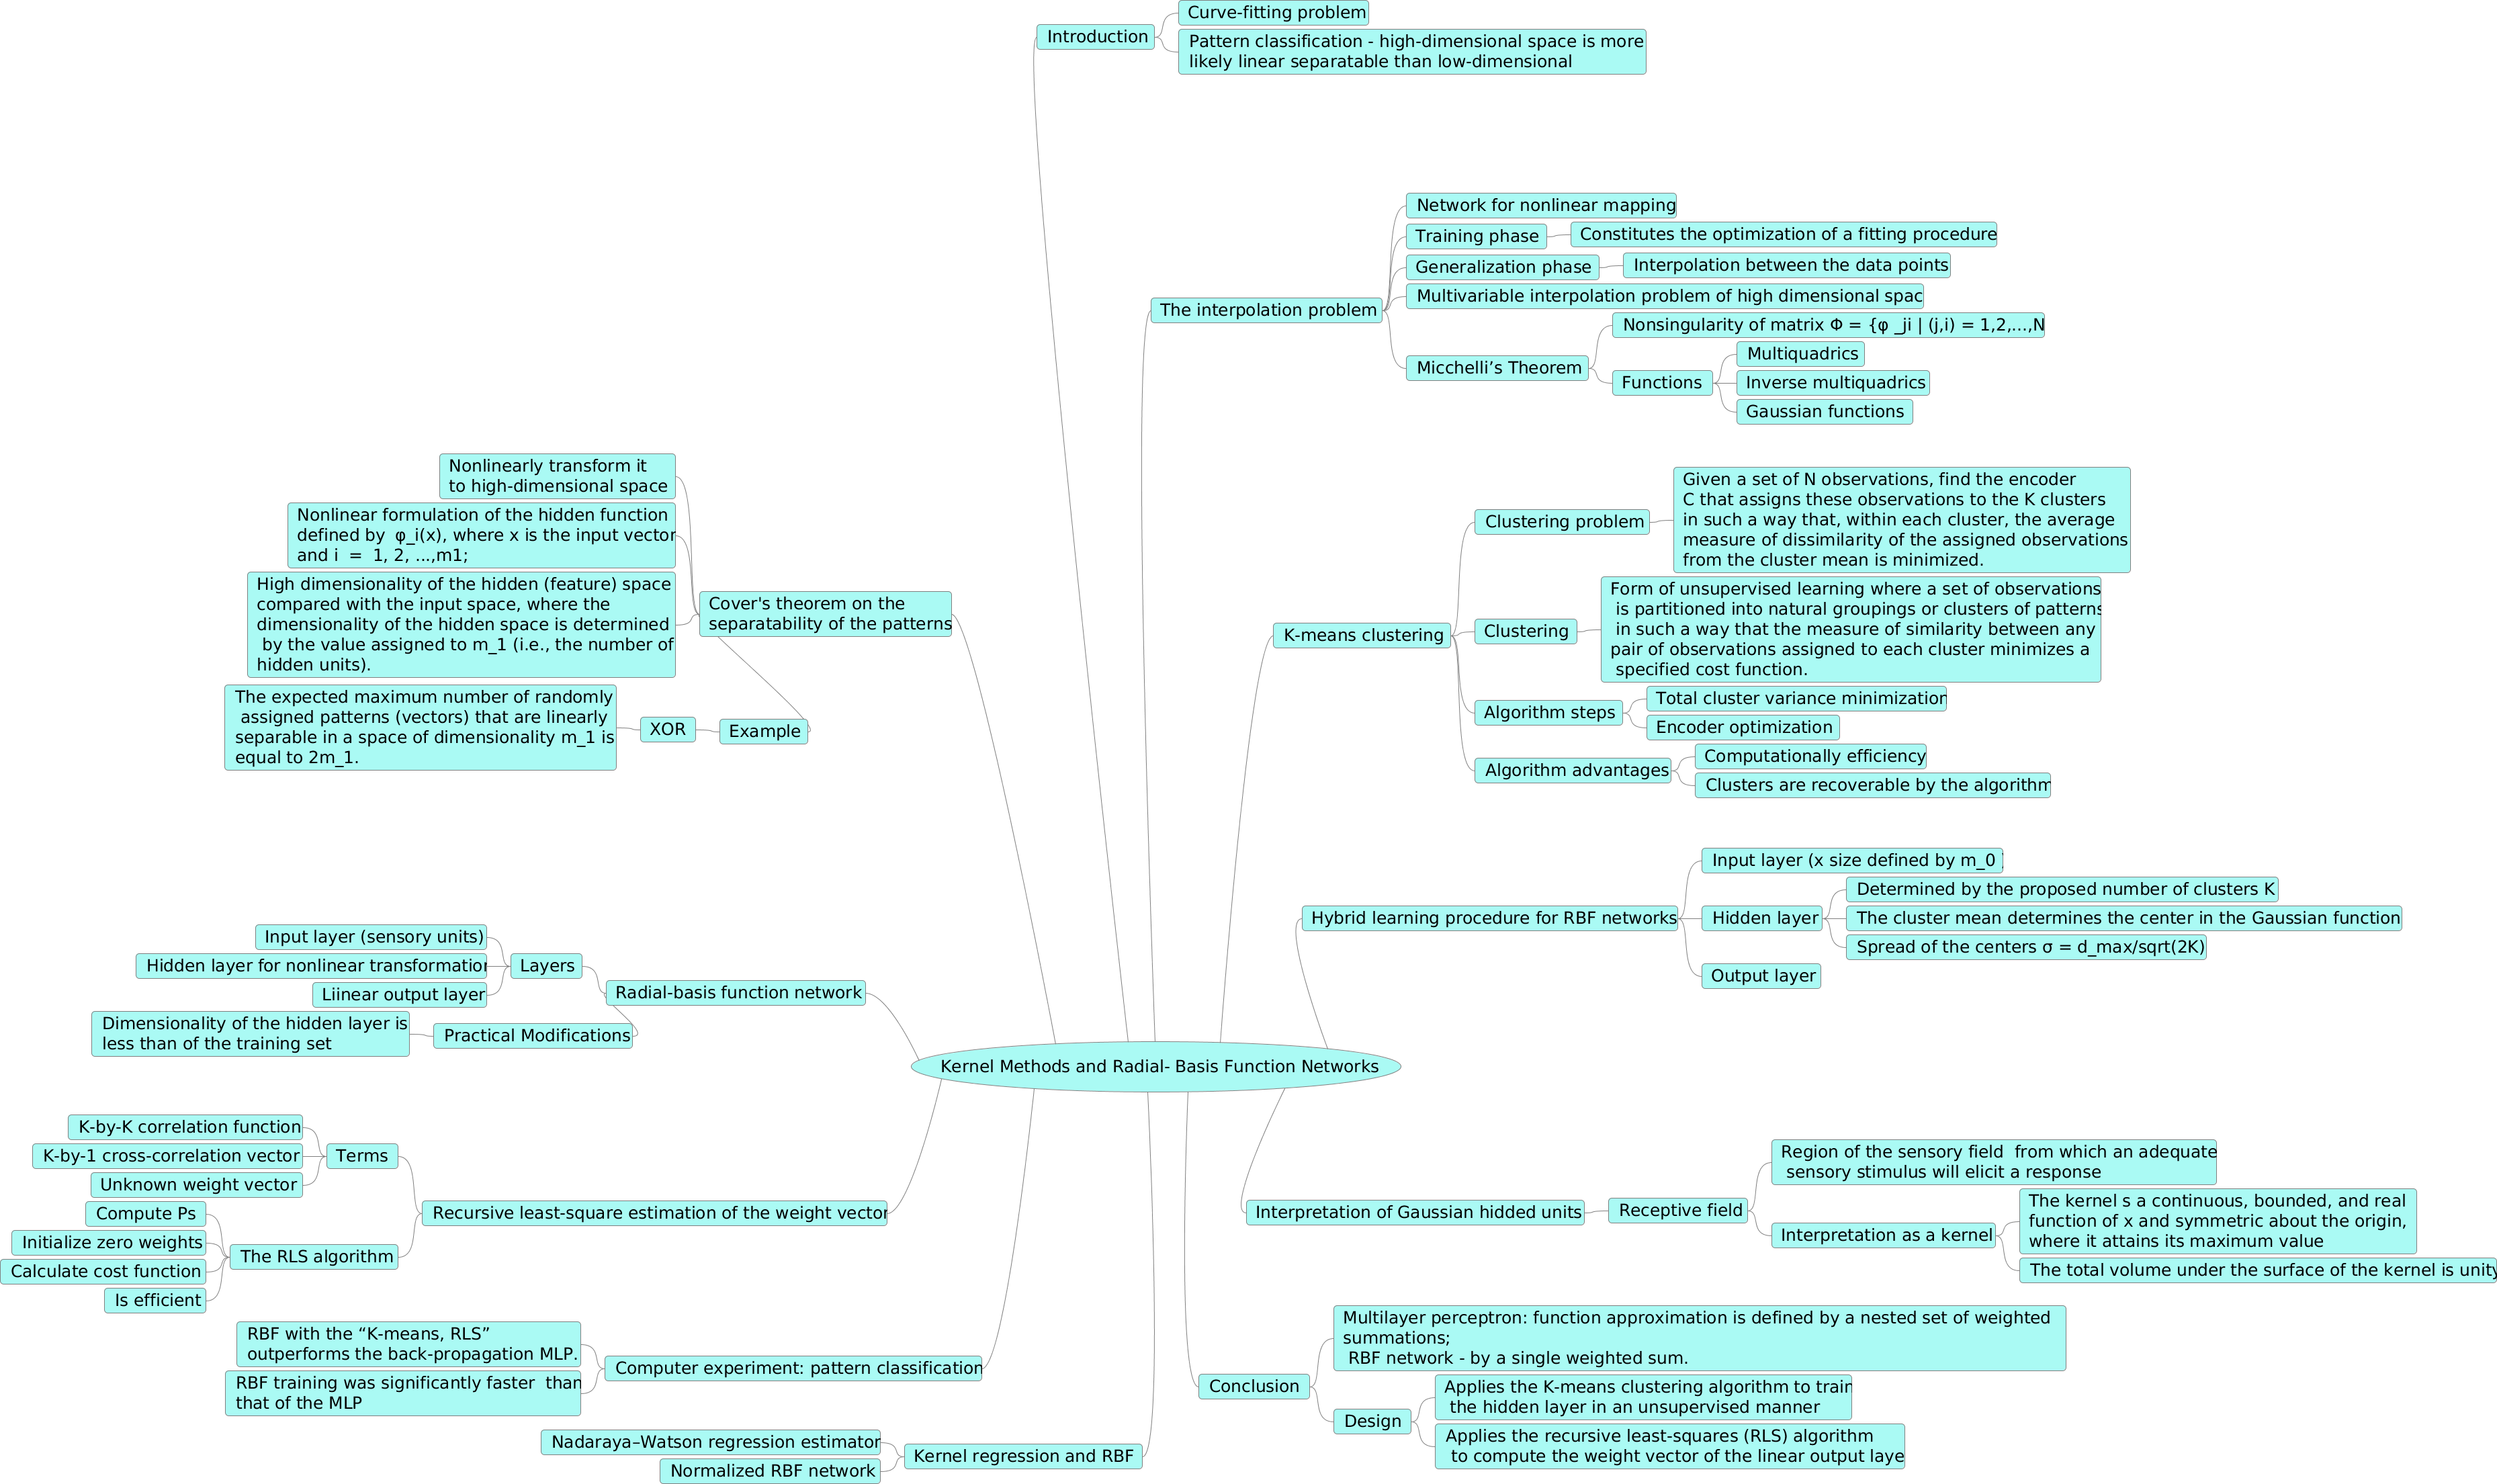
\includegraphics[width=1.0\textwidth]{Radial-BasisFunctionNetworks}
\end{figure}



\section{Exercises}

\subsection{Exercise 5.10}

The purpose of this computer experiment is to investigate the clustering process performed by the K-means algorithm. To provide insight into the experiment, we fix the number of clusters at K=6, but vary the vertical separation between the two moons in Fig. \ref{fig:moons}. Specifically, the requirement is to do the following, using an unlabled training sample of 1,000 data points picked randomly from the two regions of the double-moon pictured in Fig. \ref{fig:moons}:\\
\begin{itemize}
\item[(a)] Experimentally, determine the mean $\hat{\mu}_j$ and variance $\hat{\sigma}^2_j$, $j=1,2,..,6$, for the sequence of eight uniformly spaced vertical separations starting at $d=1$ and reducing them by one till separation $d=-6$ is reached.
\item[(b)] In light pf the results obtained in previous part, comment on how the mean $\hat{\mu}_j$ of cluster $j$ is affected by reducing the separation $d$ for $j=1,2$ and $3$.
\item[(c)] Plot the variance $\hat{\sigma}^2_j$ versus the separation $d$ for $j=1,2,...,6$.
\item[(d)] Compare the common $\sigma^2$ computed in accordance with the empirical formula of the equation $\sigma = \frac{d_{max}}{\sqrt{2K}}$ with the trends exhibited in the plots obtained in (c).
\end{itemize}

\begin{figure}[h]
  \centering
  \caption{The double moon classification problem \label{fig:moons}}
  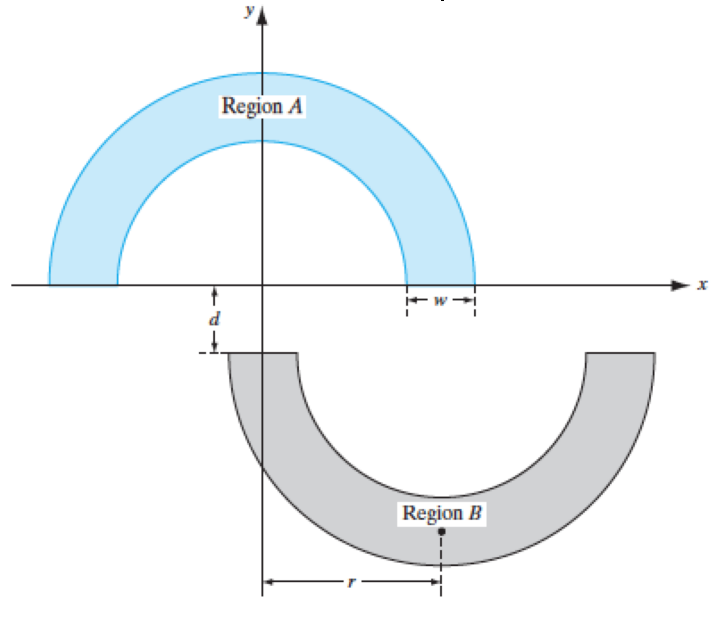
\includegraphics[width=0.5\textwidth]{moons}
\end{figure}

Solution:\\

To solve this problem first we've put some values to the moons' radiuses and w: rLarge = 30, rSmall = 23, w = 5. So, the equations to describe these moons are the following: large top circle $y = \sqrt{(30^2 - x^2)}$, small top circle $y = \sqrt{(25^2 - x^2)}$, large bottom circle $y = -d - \sqrt{(30^2 - (x - 27.5)^2)}$,  large bottom circle $y = -d - \sqrt{(25^2 - (x - 27.5)^2)}$.

\lstset{language=Python}
\begin{lstlisting}[frame=single]
import numpy as np
from sklearn.cluster import KMeans

#double moon parameters. w and radiuses are not given, so we assume that w = 5, r = 25, R = 30.
# So, the moons equations are the following:
# large top circle y = sqrt(30^2 - x^2)
# small top circle y = sqrt(25^2 - x^2)
# large bottom circle y = -d - sqrt(30^2 - (x - 27.5)^2)
# large bottom circle y = -d - sqrt(25^2 - (x - 27.5)^2)
w = 5
d = np.array([1,0,-1,-2,-3,-4,-5,-6])
r = 25
R = 30

#the moons

import matplotlib.pyplot as plt

%matplotlib inline

# evenly sampled time at 200ms intervals
t_up = np.arange(-30., 30, 0.2)
t_bot = np.arange(-2.5, 57.5, 0.2)

# red dashes, blue squares and green triangles
plt.plot(t_up, np.sqrt(R**2 - t_up**2), 'b--', t_up, np.sqrt(r**2 - t_up**2), 'b--',
    t_bot, - np.sqrt(R**2 - (t_bot - 27.5)**2) + d[7], 'r--',  t_bot, - np.sqrt(r**2 - (t_bot - 27.5)**2) + d[7], 'r--')
plt.show()
\end{lstlisting}

With these equations we get the moons depicted in Fig. \ref{fig:moonsPlot}.

\begin{figure}[h]
  \centering
  \caption{The double moon plotted with chosen parameters \label{fig:moonsPlot}}
  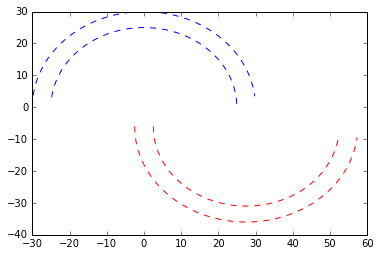
\includegraphics[width=0.5\textwidth]{moonsPlot}
\end{figure}

Then we generate the 1000 points inside these circles - by creating random arrays for the radiuses between the radius of a large ans a small circles:
\begin{lstlisting}
# train points generation
randomRad = np.random.randint(250, high=300, size=1000)/10.0
randomAngle = np.random.randint(0, high=360, size=1000)

def generate_points(d):
    X_train = np.array([[0, 27]])
    for i in range(len(randomAngle)):
        angle = math.pi*randomAngle[i]/180
        if (randomAngle[i] < 180):
            x = randomRad[i]*math.sin(angle)
            y = randomRad[i]*math.cos(angle)
        else:
            x = randomRad[i]*math.sin(angle) + 27.5
            y = randomRad[i]*math.cos(angle) - d
        point = np.array([x,y])
        X_train = np.row_stack((X_train, point))
    return X_train


X = np.array([generate_points(d[0]), generate_points(d[1]), generate_points(d[2]), generate_points(d[3]),
              generate_points(d[4]), generate_points(d[5]), generate_points(d[6]), generate_points(d[7])])
\end{lstlisting}

\textbf{(a)} After it we need to initialize centroids. We choose 6 centroids for each d randomly from the generated points:

\begin{lstlisting}
#Second step is centroids initialization. We choose 6 centroids for each d randomly from the points:
def init_centroids(X):
    centroids = np.array([])
    indices = np.random.randint(0, high=1000, size=6)
    for i in range(K):
        centroids = np.append(centroids, X[indices[i]])
    return centroids.reshape(K,2)
centroids = np.array([])
for i in range(len(d)):
    centroids = np.append(centroids,init_centroids(X[i]))
print centroids.reshape(len(d),K,2)


[[[ 24.0315424    6.8909339 ]
  [ 17.37620376  28.81490158]
  [ 14.00600244 -21.45778328]
  [  4.13496686  10.44008615]
  [ 23.11084857 -10.77676567]
  [ 27.13230009 -12.0800783 ]]

...

 [[ 28.2827604    0.98765576]
  [  0.42616763   4.39267054]
  [  0.33280959 -16.42850733]
  [  2.83046993 -16.47159424]
  [  1.00403608  -5.53751123]
  [ 16.23646609  20.05036581]]]


 plt.grid(True)
plt.plot(X[1][:,0], X[1][:,1], 'r^', centroids[0][:,0],centroids[0][:,1], 'bo')
plt.show()

plt.grid(True)
plt.plot(X[7][:,0], X[7][:,1], 'g^', centroids[7][:,0],centroids[7][:,1], 'bo')
plt.show()
\end{lstlisting}

The centroids for first and last ds are depicted in Fig. \ref{fig:centr}.

\begin{figure}[h]
  \centering
  \caption{The double moon (red - for d = 1 and green - for d = -6 triangles) with centroids (blue points) \label{fig:centr}}
  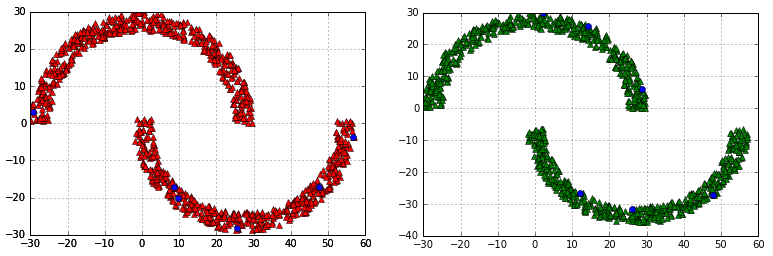
\includegraphics[width=0.8\textwidth]{centr}
\end{figure}

The next step is to assign points to clusters by finding the shortest distance between the points and clusters:
\begin{lstlisting}
import scipy.spatial.distance
#find the closest to centroids points
def assign_points_to_centroids(X, centroid_set):
    shortest = np.array([])
    distancies = scipy.spatial.distance.cdist(X, centroid_set)
    for i in range(len(distancies)):
        point_to_cluster = np.array([np.argmin(distancies[i]), np.amin(distancies[i])])
        shortest = np.append(shortest, point_to_cluster)
    return shortest.reshape(len(distancies), 2)

points_in_clusters = np.array([])
for i in range(len(d)):
    points_in_clusters = np.append(points_in_clusters, assign_points_to_centroids(X[i], centroids[i]))
points_in_clusters = points_in_clusters.reshape(len(d), len(X[0]), 2)
print points_in_clusters


[[[  3.           8.01371165]
  [  0.          23.24707832]
  [  1.          32.58619713]
  ...,
  [  4.           8.02426658]
  [  5.          10.33305738]
  [  0.           3.52343674]]

...

 [[  1.           3.42927548]
  [  0.          13.41239277]
  [  3.          18.72193546]
  ...,
  [  0.           3.43011793]
  [  1.          12.20407394]
  [  5.           3.42414427]]]
\end{lstlisting}

And then follows the actual learning. We need to move centroids in such a way that they would 	be in the middle of the point cloud assigned to them:\\

\begin{lstlisting}
def centroids_moving(X, points_in_clusters, centroid_set):
    return np.array([X[points_in_clusters[:,0] == k].mean(axis=0) for k in range(len(centroid_set))])
new_position_centr = np.array([])
for i in range(len(d)):
    new_position_centr = np.append(new_position_centr, centroids_moving(X[i], points_in_clusters[i], centroids[i]))
new_position_centr = new_position_centr.reshape(len(d),K,2)
print new_position_centr

[[[-13.82919874  19.64638503]
  [ 44.62527485 -17.08127271]
  [ 49.2583624   -2.58098819]
  [ 12.81568895   5.20702855]
  [ 26.75005756 -25.69362956]
  [ 13.03522465 -21.93359926]]
...
 [[ 15.65318603  18.39961297]
  [-23.20695024  12.64083583]
  [  9.79272096 -22.96052392]
  [ 31.122512   -32.82182453]
  [ 48.62381334 -21.15032426]
  [-10.3448574   24.93610957]]]
\end{lstlisting}

Using previous step update the centroids coordinates till the difference between new and old ones is less than 0.1:

\begin{lstlisting}
new_position_centr = np.array([])
iterations = np.array([])
for i in range(len(d)):
    iter = 0
    old_position_centr = centroids[i]
    dists = 100
    cluster_points = assign_points_to_centroids(X[i], old_position_centr)
    while(dists > 0.1):
        iter+=1
        #update cluster
        new_position_c = centroids_moving(X[i], cluster_points, old_position_centr)
        #update points
        cluster_points = assign_points_to_centroids(X[i], new_position_c)
        dists = 0
        for j in range(K):
            dists += scipy.spatial.distance.euclidean(old_position_centr[j], new_position_c[j])
        old_position_centr = new_position_c
    iterations = np.append(iterations, iter)
    new_position_centr = np.append(new_position_centr, new_position_c)

new_position_centr = new_position_centr.reshape(len(d),K,2)
print "iterations"
print iterations
print "centroids"
print new_position_centr

iterations
[ 24.  30.  25.   8.  17.  12.  11.   7.]
centroids
[[[ 49.40952006 -12.93490955]
  [-21.9539597   14.08117102]
  [ 25.82518642 -25.17856609]
  [ 23.05741957  12.17402433]
  [  4.14254172 -11.15832509]
  [  0.45427766  26.09350205]]

 ...

 [[  4.98230105 -19.26547119]
  [ 50.47929746 -18.7701339 ]
  [  2.37019789  25.9815445 ]
  [ 28.61314336 -32.18748749]
  [ 23.42569304  11.6670059 ]
  [-21.33635336  14.82847459]]]
\end{lstlisting}

The resulting centroids for the first and last ds are shown in Fig. \ref{fig:centrFin}. \\

\begin{figure}[h]
  \centering
  \caption{The double moon (red - for d = 1 and green - for d = -6 triangles) with final calculated centroids (blue points) \label{fig:centrFin}}
  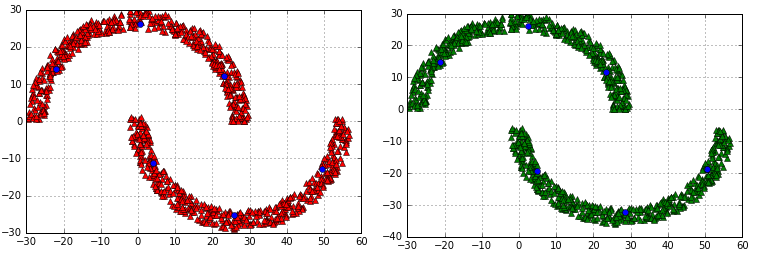
\includegraphics[width=0.8\textwidth]{centrFin}
\end{figure}

\textbf{(a)} For mean and variance calculation we used the following code:

\begin{lstlisting}
#a mean and variance calculation

def pair_dist(arr1, arr2):
    summ = 0;
    for i in range(len(arr1)):
        summ += scipy.spatial.distance.euclidean(arr1[i], arr2)
    return summ/len(arr1)
def var_for_cluster(arr1, arr2, mean):
    summ = 0;
    for i in range(len(arr1)):
        summ += (scipy.spatial.distance.euclidean(arr1[i], arr2) - mean)**2
    return summ/(len(arr1) - 1)

def mean_calculation(X, points_in_clusters, centroid_set):
    return np.array([pair_dist(X[points_in_clusters[:,0] == k], centroid_set[k]) for k in range(len(centroid_set))])

def variance_calculation(X, points_in_clusters, centroid_set, mean):
    return np.array([var_for_cluster(X[points_in_clusters[:,0] == k], centroid_set[k], mean[k]) for k in range(len(centroid_set))])

mean = np.array([])
variance = np.array([])
for i in range(len(d)):
    points = assign_points_to_centroids(X[i], new_position_centr[i])
    mean_tmp = mean_calculation(X[i], points, new_position_centr[i])
    mean = np.append(mean, mean_tmp)
    variance_tmp = variance_calculation(X[i], points, new_position_centr[i], mean_tmp)
    variance = np.append(variance, variance_tmp)
mean = mean.reshape(len(d), len(mean_tmp))
variance = variance.reshape(len(d), len(variance_tmp))
print mean
print variance
\end{lstlisting}

So, we've obtained the following means : [[  8.11551501   6.89620468   7.05776613   7.38103096   7.7538904
    7.69813644]
 [  5.45685966   5.78160551   4.91614198  10.67401462  10.94663218
    5.7996544 ]
 [ 10.94663218  10.67401462   5.7996544    4.91614198   5.45685966
    5.78160551]
 [  5.12399471   5.9802248   10.83794335  10.47906663   5.65293167
    5.31845917]
 [  5.96931319  10.83794335   5.03875964   5.58564629   5.44074919
   10.47906663]
 [  5.52657573   4.91614198  10.67401462   5.70120506  10.94663218
    5.7996544 ]
 [  7.7538904    7.05776613   7.31133375   7.46133993   8.11551501
    7.25492557]
 [  7.31133375   8.29599059   7.46133993   6.74378599   7.25492557
    7.71256627]]\\

and variances:\\

[[ 14.62263462  16.0437904   14.86025695  15.14036738  12.38129185
   15.15804983]
 [  7.84305872  10.28209152   6.38976484  29.80877893  26.90941454
    9.23635644]
 [ 26.90941454  29.80877893   9.23635644   6.38976484   7.84305872
   10.28209152]
 [  6.0968976    7.93027525  32.81736714  27.11795529   8.33838342
    7.67798775]
 [  8.42205311  32.81736714   5.78362442   7.97020471   8.42114792
   27.11795529]
 [  8.15256191   6.38976484  29.80877893  10.01222759  26.90941454
    9.23635644]
 [ 12.38129185  14.86025695  13.81686673  17.58098457  14.62263462
   13.80546138]
 [ 13.81686673  14.57946065  17.58098457  13.62149918  13.80546138
   14.16774844]]\\
for ($d_1 - d_8$).

\textbf{(b)} In Fig. \ref{fig:mean} we show the mean - d dependency.

\begin{lstlisting}
#b
plt.xlabel('d')
plt.ylabel('mean[j]')
colors = ['b--', 'g--', 'r--']

for i in range(3):
    plt.plot(d, mean[:,i], colors[i])
plt.show()
\end{lstlisting}

\begin{figure}[h]
  \centering
  \caption{Blue - $\hat{\mu}_1$ , green - $\hat{\mu}_2$ , red - $\hat{\mu}_3$ , \label{fig:mean}}
  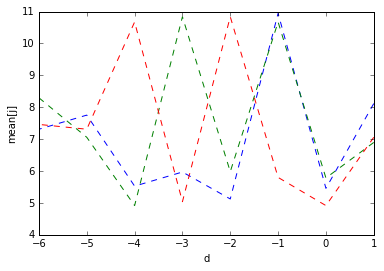
\includegraphics[width=0.6\textwidth]{mean}
\end{figure}

The mean values show symmetry.

\textbf{(c)}  See Fig. \ref{fig:variance}.

\begin{lstlisting}
#c
plt.xlabel('d')
plt.ylabel('variance[j]')
colors = ['b--', 'g--', 'r--', 'c--', 'm--', 'k--']

for i in range(6):
    plt.plot(d, variance[:,i], colors[i])
plt.show()
\end{lstlisting}


\begin{figure}[h]
  \centering
  \caption{Blue - $\hat{\sigma}_1^2$, green - $\hat{\sigma}_2^2$, red - $\hat{\sigma}_3^2$, cian - $\hat{\sigma}_4^2$, magenta - $\hat{\sigma}_5^2$, black - $\hat{\sigma}_6^2$ \label{fig:variance}}
  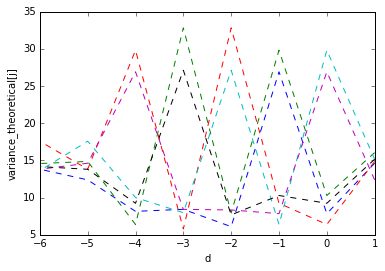
\includegraphics[width=0.6\textwidth]{sigmaTh}
\end{figure}

\textbf{(d)}  In Fig. \ref{fig:sigmaTh} we show the theoretical $\sigma^2$ and experimental $\hat{\sigma}^2$s.

\begin{figure}[h]
  \centering
  \caption{Blue - $\hat{\sigma}_1^2$, green - $\hat{\sigma}_2^2$, red - $\hat{\sigma}_3^2$, cian - $\hat{\sigma}_4^2$, magenta - $\hat{\sigma}_5^2$, yellow - - $\hat{\sigma}_6^2$ ,black - $\hat{\sigma}_theor$ \label{fig:sigmaTh}}
  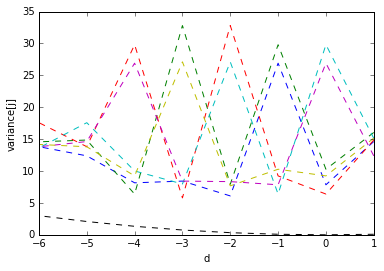
\includegraphics[width=0.6\textwidth]{variance}
\end{figure}


\subsection{Exercise 5.11}
The purpose of this second experiment is to compare the classification performance of two hybrid learning algorithms: the "K-means,RLS" algorithm investigated in Section 5.8 and the "K-means,LMS" algorithm investigated in this problem.\\
	As in section 5.8, assume the following:\\
Number of hidden Gaussian units:20\\
Number of training samples:1,000 data points\\
Number of testing samples: 2,000 data points\\
Let the learning-rate parameter of the LMS algorithm be annealed linearly from 0.6 down to 0.01.
\begin{itemize}
\item[(a)] Construct the decision boundary computed for the "K-means,LMS" algorithm for the vertical separation between the two moons in Fig.\ref{fig:moons} set at $d=-5$.
\item[(b)] Repeat the experiment for $d=-6$.
\item[(c)] Compare the classification results obtained using the "K-means,LMS" algorithm with those of the "K-means,RLS" algorithm studied in Section 5.8.
\item[(d)] Discuss how, in general, the complexity of the "K-means,LMS" algorithm compares with that of the "K-means,RLS" algorithm.
\end{itemize}

\subsection{Exercise 3}
Repeat the Ex3 from the previous assignment with the Radial Basis Functions. Investigate the use of Radial Basis Functions to achieve one-to-one mappings, as described here:
\begin{enumerate}
\item $F(x) = 1/x 1<=x<=100$

\item $F(x) = log10(x) 1<=x<=10$

\item $F(x) = exp(-x) 1<=x<=10$

\item $F(x) = sin(x) 0<=x<=pi/2$
\end{enumerate}
For each mapping, do the following:
\begin{itemize}
\item Set up two sets of data, one for network training, and the other for testing.

\item Use the training data set to compute the synaptic weights of the network, assumed to have a single hidden layer.

\item Evaluate the computation accuracy of the network by using the test data. Use a single hidden layer but with a variable number of hidden neurons. Investigate how the network performance is affected by varying the size of the hidden layer.
\end{itemize}
For solving this problem or you have to use your own implementation.

\subsubsection{Solution}

Radial Basis Function NN was implemented in MATLAB and has 2 functions:
\begin{itemize}
\item evaluation of RBF NN on given data array;

\item Training of the RBF NN.
\end{itemize}

The algorithm works for RBF NN with chosen number of neurons in a hidden layer. Centroids of the RBF can be initialized uniformly distributed or with fixed step size grid. Sigma values are chosen based on distance to 2 nearest centroids.
\medskip
Matlab code for RBF NN training:

\lstinputlisting{trainRBF.m}

\subsubsection{Experimental results}

The NN can easily mimic nonlinear functions. Random centroids shows better performance that fixed step size grid. Usually, the error goes to machine zero. 

Results of the experiments:
\begin{enumerate}
\newpage
\item $1/x$ function with uniform centroids.

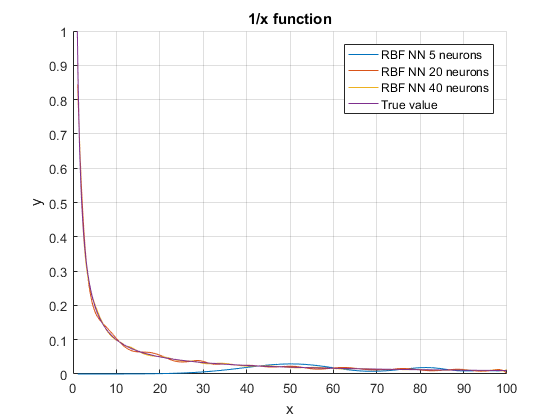
\includegraphics[scale = 0.8]{f11.png}

\item $1/x$ function with grid centroids.

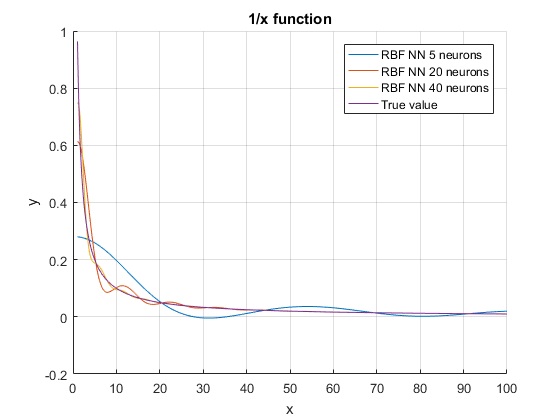
\includegraphics[scale = 0.8]{f1.png}
\newpage
\item $log_{10}$ function with uniform centroids.

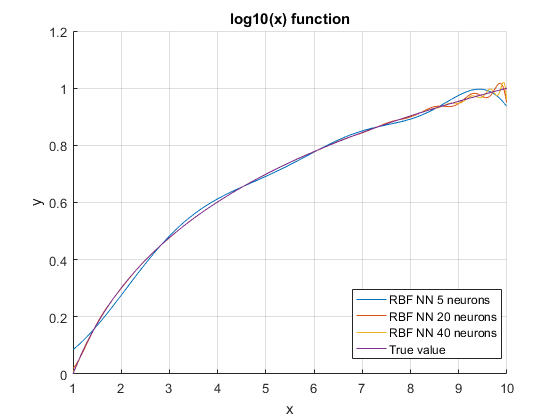
\includegraphics[scale = 0.8]{f2.png}

\item $log_{10}$ function with grid centroids.

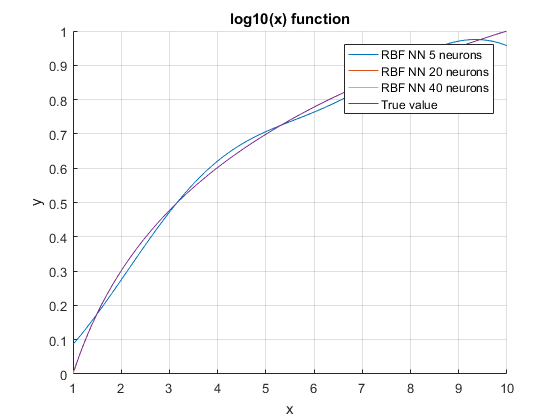
\includegraphics[scale = 0.8]{f22.png}
\newpage
\item $\exp(-x)$ function with uniform centroids.

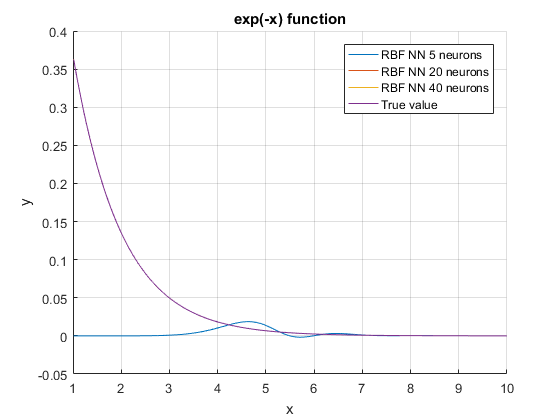
\includegraphics[scale = 0.8]{f33.png}

\item $\exp(-x)$ function with grid centroids.

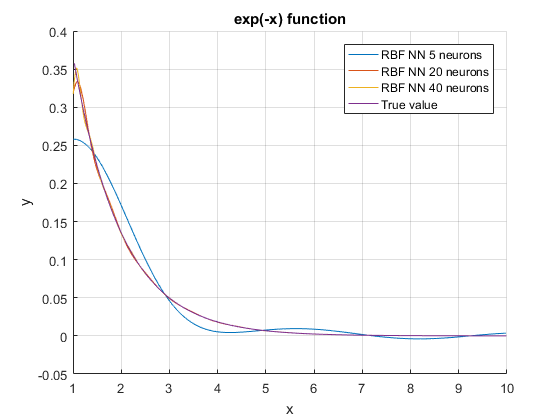
\includegraphics[scale = 0.8]{f3.png}
\newpage
\item $\sin(x)$ function with uniform centroids.

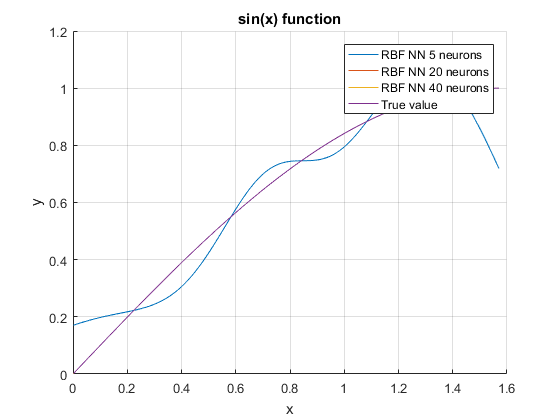
\includegraphics[scale = 0.8]{f44.png}

\item $\sin(x)$ function with grid centroids.

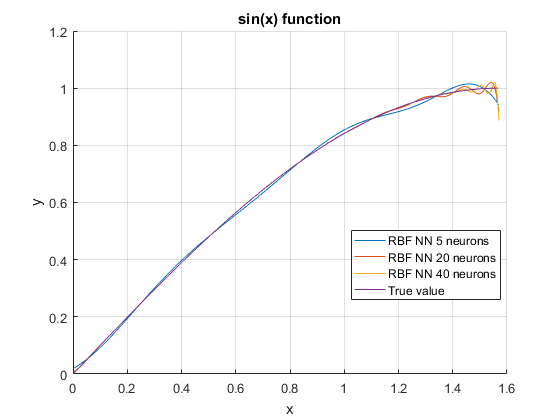
\includegraphics[scale = 0.8]{f4.png}


\end{enumerate}

Dependency of error based on number of hidden neurons:

\begin{enumerate}
\newpage
\item $1/x$ function with uniform centroids.

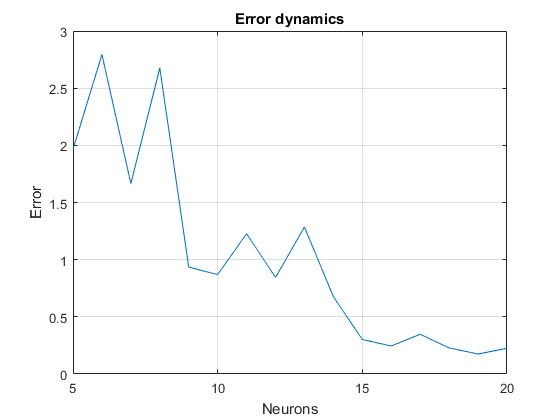
\includegraphics[scale = 0.8]{e11.png}

\item $1/x$ function with grid centroids.

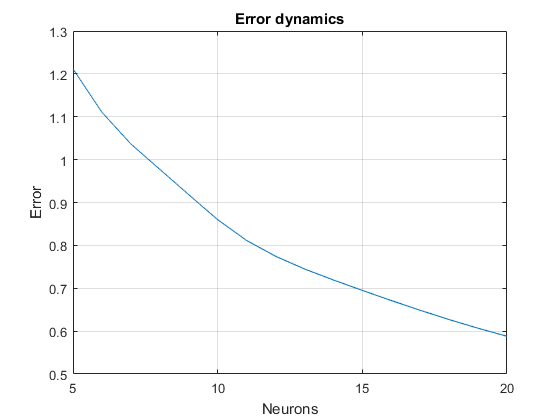
\includegraphics[scale = 0.8]{e1.png}
\newpage
\item $log_{10}$ function with uniform centroids.

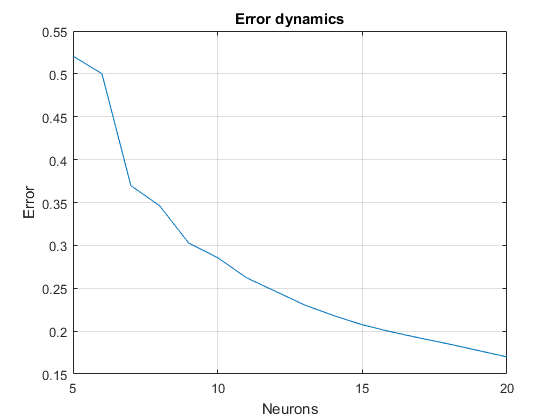
\includegraphics[scale = 0.8]{e2.png}

\item $log_{10}$ function with grid centroids.

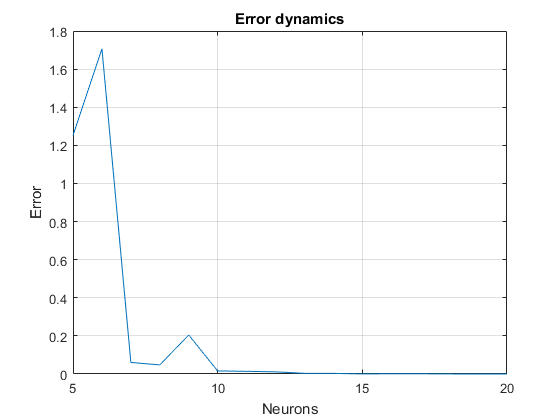
\includegraphics[scale = 0.8]{e22.png}
\newpage
\item $\exp(-x)$ function with uniform centroids.

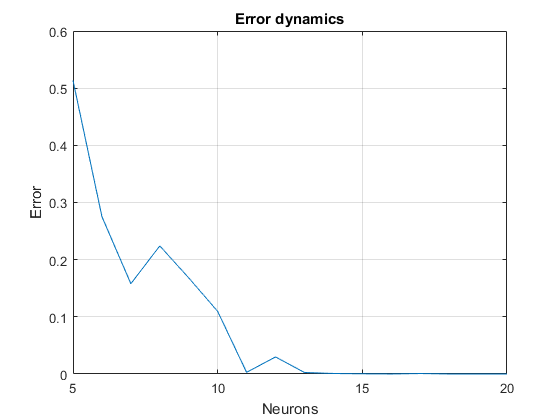
\includegraphics[scale = 0.8]{e33.png}

\item $\exp(-x)$ function with grid centroids.

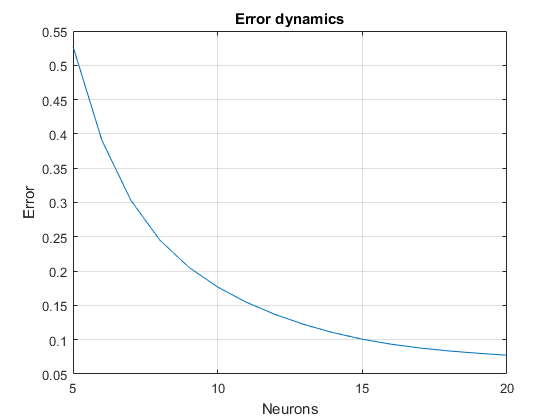
\includegraphics[scale = 0.8]{e3.png}
\newpage
\item $\sin(x)$ function with uniform centroids.

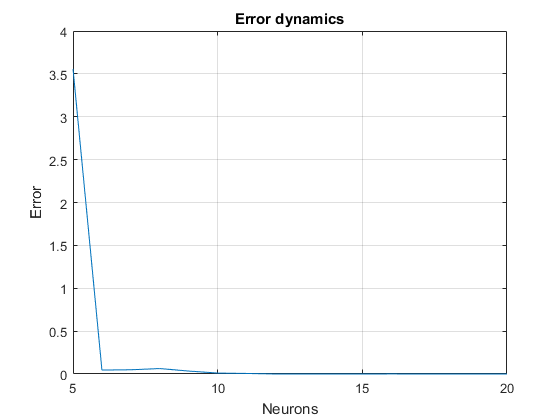
\includegraphics[scale = 0.8]{e44.png}

\item $\sin(x)$ function with grid centroids.

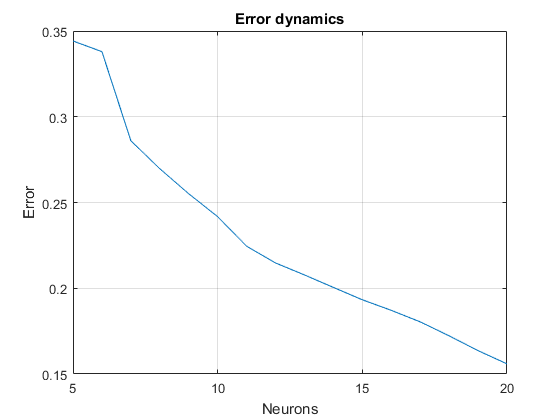
\includegraphics[scale = 0.8]{e4.png}


\end{enumerate}
The error decreases dramatically with extra neurons in a hidden layer.

\end{document}
